\documentclass[10pt, oneside,spanish]{article}   	
\usepackage{geometry}                		
\geometry{a4paper}                   		
\usepackage[spanish, es-noindentfirst]{babel}
\selectlanguage{spanish}
\usepackage[utf8]{inputenc}               		
\usepackage{amsmath}    		
\usepackage{graphicx}				
\graphicspath{ {/home/user/images/} }										
\usepackage{amssymb}
\usepackage{authblk}
\usepackage{algorithmic}
\usepackage{algorithm}
\usepackage{listings}
\usepackage[nottoc]{tocbibind}

\title{Implementación de la Factorización Cholesky con openMP}
\author[1]{Alejandro Nivón}
\author[2]{Uriel Miranda}
\author[3]{Héctor Corro}
\affil[ ]{Maestría en Ciencia de Datos}
\affil[ ]{Instituto Tecnológico Autónomo de México}
\renewcommand\Authands{, }
\date{}							

\begin{document}
\maketitle

\section{Introducción}
   
\textbf{Objetivo:}
aprovechar las oportunidades creadas o generadas por las tecnologías actuales para la paralelización de rutinas del cálculo numérico, para cuestiones de este trabajo y para la implementación de alguna de los paradigmas de programación vistos en la clase de Análisis Numérico y Computo Científico. Se hará uso de openMP para la factorización Cholesky aprovechando las siguientes características de openMP: 


\begin{itemize}
\item Paralelización for-loops secuenciales de forma simple
\end{itemize}
\begin{itemize}
\item Paralelización de tarea y sincronización explícita de threads
\end{itemize}
\begin{itemize}
\item Permite una paralelización del código secuencial de forma paulatina (incremental paralellism)
\end{itemize}

\textbf{Factorización Cholesky} Una matriz simétrica $nxn$ $A$ es positiva definida si su forma cuadrática $X^TAX$ es positiva definida para todos los vectores no-cero $x$ o, equivalentemente si todos los eigenvalores de $A$ son positivos.
Las matrices positivas definidas pueden ser expresadas de la forma $A = X^TX$ para una matriz $X$ no singular.
La factorización Cholesky es una forma particular de factorizar $X$, en la que $X$ es la matriz triangular superior con elementos positivos en su diagonal; generalmente es escrito como: \(A = R^TR\) o $A = LL^T$ de una matriz definida \(A\), en la que \(R\) es una matriz triangular superior con elementos positivos en su diagonal es una herramienta fundamental para la computación matricial.
El algoritmo estándar para su cómputo data de principios del siglo pasado y es uno de los métodos numéricos más estables de todos los algoritmos matriciales. 
La factorización Cholesky existe y es única si A es positiva definida. \cite{choi1996design}
 

\textbf{Lemma 1.1:}
Sea \(A\) positiva semi-definida de rango \(r\).

\begin{enumerate}
\item Existe al menos una matriz triangular superior \(R\) con elementos no negativos en su diagonal tal que \(A = R^TR\).
\end{enumerate} 

\begin{enumerate}
\item Hay una permutación $\prod$ tal que $\prod^TA\prod$ tiene una única factorización cholesky que toma la forma: 
\end{enumerate}

\begin{equation}
\prod^TA\prod = R^TR ,
\end{equation}

\[
R = 
 \begin{pmatrix}
  r_{1,1} & r_{1,2} \\
  0 & 0
 \end{pmatrix}
\]

\section{Aplicaciones}
La descomposición de Cholesky se usa principalmente para hallar la solución numérica de ecuaciones lineales $Ax = b$. Si $a$ es simétrica y positiva definida, entonces se puede solucionar $Ax = b$ calculando primero la descomposición de Cholesky $A = LL^T$, luego resolviendo $Ly = b$ para $y$, y finalmente resolviendo $L^Tx = y$ para $x$.

\begin{itemize}
\item \textbf{Mínimos cuadrados lineales:}
\end{itemize}

Sistemas de la forma $Ax =b$ con $A$ simétrica y definida positiva aparecen a menudo en la práctica. Por ejemplo las ecuaciones normales en problemas de mínimos cuadrados lineales son problemas de esta forma. 

\begin{itemize}
\item \textbf{Simulación de Montecarlo:}
\end{itemize}

La descomposición de cholesky se usa comúnmente en el método de Montecarlo para simular sistemas con variables múltiples correlacionadas: la matriz de correlación entre variables es descompuesta, para obtener la triangular inferior $L$. Aplicando ésta un vector de ruidos simulados incorrelacionados, $u$ produce un vector $Lu$ con las propiedades de covarianza del sistema a ser modelado.

\begin{itemize}
\item \textbf{Filtro de Kalman:}
\end{itemize}

Los filtros de Kalman usan frecuentemente la descomposición de Cholesky para escoger un conjunto de puntos sigma. El filtro de Kalman sigue el estado promedio de un sistema como un vector $x$ de longitud $n$ y covarianza dada por una matriz $P$ de tamaño $nxn$. La matriz $P$ es siempre semidefinida positiva y puede descomponerse como $LL^T$. Las columnas de $L$ pueden ser adicionadas y restadas de la media $x$ para formar un conjunto de $2N$ vectores llamados puntos sigma. Estos puntos sigma capturan la media y la covarianza del estado del sistema.

\begin{itemize}
\item \textbf{Estabilidad del proceso de Cholesky}
\end{itemize}

En aritmética exacta se sabe que una matriz simétrica positiva definida tiene una factorización Cholesky. Asimismo, si el proceso Cholesky que se mostrará posteriormente en este trabajo realiza su iteración hasta su terminación con raíces cuadradas estrictamente positivas, entonces la matriz A es positiva definida.
Por lo tanto, para encontrar si una matriz $A$ es positiva definida, solamente se intentará de computar la factorización Cholesky usando el método citado a continuación.

\section{Calculo}

La Factorización Cholesky puede ser calculada por una forma de eliminación gaussiana que toma ventaja de la simetría y definición. Iterando $(i,j)$, elementos en la ecuación $A = R^TR$ como se ve a continuación:

\begin{equation}
\j = i \qquad a_{ii} = {\displaystyle\sum_{k=1}^{i}{r^2_{ki}}}
\end{equation}

\begin{equation}
\j>i \qquad a_{ij} = {\displaystyle\sum_{k=1}^{i}{r_{ki}}{r_{kj}}}
\end{equation}

Estas ecuaciones pueden ser resueltas para producir $R$ columnas a la vez, de acuerdo con el siguiente algoritmo:

\begin{figure}[h]
    \centering
    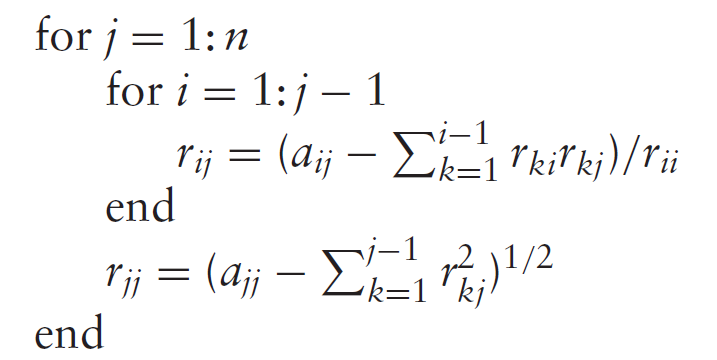
\includegraphics[width=0.5\textwidth]{for_cycle}
    \caption{Algoritmo: Factorización Cholesky}
    \label{fig:mesh1}
\end{figure}

Que $A$ sea positiva definida garantiza que el argumento de la raíz cuadrada en este algoritmo es siempre positivo y por lo tanto que $R$ tiene una diagonal positiva. Este algoritmo requiere $n^3/{3 + O(n^2)}$ flops y $n$ raíces cuadrada, donde un flop es cualquiera de las 4 operaciones aritméticas elementales escalares $+,-,*$ y $/$. \cite{golub2012matrix}

\section{Algoritmo}
\textbf{Algoritmo:}
Después de investigar diferentes aproximaciones y formas de desarrollar la factorización de Cholesky, así como su implementación, se decidió paralelizar con base en el cálculo de filas. Para esto lo más importante a considerar es el orden en que se realizan los cálculos.

Regresando al algoritmo original de la factorización de Cholesky se tienen dos fórmulas, una para los elementos en la diagonal y otra para los elementos bajo la diagonal. \cite{higham1990analysis}


\begin{itemize}
\item \textbf{Elementos en la diagonal}
\end{itemize}

\begin{equation}
\L_{ij}=\sqrt{A_{ij} - {\displaystyle\sum_{k=1}^{j-1} L^2_{jk}}} 
\end{equation}

\begin{itemize}
\item \textbf{Elementos bajo la diagonal}
\end{itemize}

\begin{equation}
\L_{ij} = \frac{1}{L_{jj}} \big( A_{ij} - {\displaystyle\sum_{k=1}^{j-1} L_{ik}L_{jk}}\big)
\end{equation}

El algoritmo para realizar el proceso de manera paralela se deriva de la forma y dependencia de los elementos que se requieren para realizar el cálculo de cada uno de los elementos.
Iniciando por el elemento $l_{11}$:

Aplicando la fórmula para elementos en la diagonal, tenemos:

\begin{equation}
\l_{11} = \sqrt{a_{11}}
\end{equation}

Para calcular el elemento $l_{21}$:

\begin{equation}
\l_{21} = \sqrt{a_{21}}
\end{equation}

Por lo cual para cada elemento de la columna j=1 no requiere dependencia de ningún otro elemento, por lo cual se puede realizar en paralelo.

Siguiendo con esa línea para calcular el elemento $l_{32}$

\begin{equation}
\l_{32} = \frac{1}{l_{33}} \big( a_{32} - {l_{31}l_{21}}\big)
\end{equation}

Comparamos con el cálculo del elemento  $l_{42}$:

\begin{equation}
\l_{42} = \frac{1}{l_{44}} \big( a_{42} - {l_{41}l_{21}}\big)
\end{equation}

La dependencia de elementos de la matriz L para los dos elementos de la misma columna es:

\begin{center}
	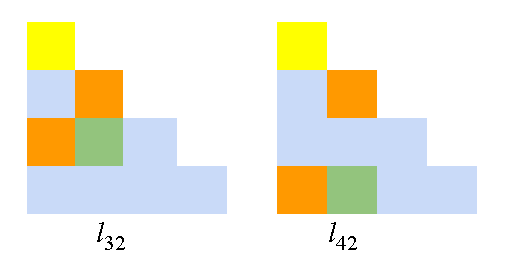
\includegraphics{MatrixGreen}
\end{center}


Los colores en este caso tienen los siguientes distintivos:

\begin{itemize}
\item Verde: El elemento que se está calculando.
\end{itemize}

\begin{itemize}
\item Naranja: Los elementos de los que depende directamente el elemento calculado.
\end{itemize}

\begin{itemize}
\item Amarillo: Los elementos de los que depende indirectamente el elemento calculado.
\end{itemize}


Con los ejemplos anteriores podemos ver que solamente se requiere el cálculo de los elementos de la fila (anteriores a la columna del elemento que se desea calcular) y el elemento que cruza con la diagonal de la misma columna.

El algoritmo para el cálculo en paralelo será:

\begin{enumerate}
\item Se calcula el elemento de la diagonal  $l_{kk}$.
\item Se calculan en paralelo los elementos para cada i con la j fija.
\item Se repite para toda $k <=n$ donde $n$ es la dimensión de la matriz, dado que es simétrica tendremos matrices de $nxn$.
\end{enumerate}

En el primer punto el cálculo depende únicamente de los elementos de la fila $k$, en una matriz de $n=5$ el orden de cálculo será:

\begin{center}
	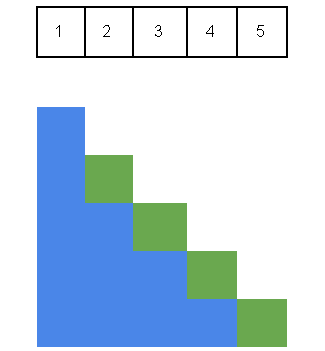
\includegraphics{MatrixBlue}
\end{center}

El orden es de $1 \to 5$ y empezando por el elemento en verde, siendo los elementos en azul ,para cada columna, los que se podrán calcular en paralelo. \cite{higham2009cholesky}

\section{Implementación}

Después de analizar los algoritmos vistos anteriormente estos se implementaron en C y OpenMP para explotar las características de esta API. Una de las caracteristicas corresponde a la forma simple de establecer que un bloque de código sea ejecutado en paralelo, algunas otras se citan a continuación:

\begin{itemize}
\item Paralelizar for-loops secuenciales de forma simple
\item Paralelización de tareas y sincronización explícita de threads
\item Permite una paralelización del código secuencial de forma paulatina (incremental paralellism)
\end{itemize}

\textbf{Algunas observaciones de OpenMP:} openMP es una API que provee de directivas para shared-memory. En términos de C, esto significa que se tiene instrucciones  especiales para el procesador. Para openMP se usa $\#pragma$. Los pragmas son añadidos al sistema para permitir comportamientos que no son parte de la especificación básica de C. Los pragmas de openMP siempre comienzan con: $\#pragma \enspace omp$.

\begin{enumerate}
\item Se diseñó y programó en R un script que genera matrices para su posterior implementación de la Factorización Cholesky en C.
	\begin{itemize}
	\item El nombre del archivo que contiene el script es \textbf{matriz.r}.
	\item Se ejecuta con el comando: python \textbf{matriz.r n}, en el cual se debe sustituir \textbf{n} por la dimensión de la matriz cuadrada positiva definida a generar.
	\item El resultado se almacenará en el archivo \textbf{matrizSPD.txt} en una sola columna, para después ser el insumo del algoritmo de factorización de cholesky con \textbf{chlesky$\_$final.c}.
	\end{itemize}
\item El script \textbf{cholesky$\_$final.out} realizará mediante standar input la ingesta de los elementos de la matriz y posteriormente imprimir la matriz factor en el archivo: \textbf{fact.txt}. Se dejan los archivos .txt como ejemplo con matrices de dimensión $20 x 20$. 
\item Por último los scripts \textbf{cholesky$\_$1.c} y \textbf{chol$\_$seq.c} son ejemplos de aplicaciones de matrices pequeñas en el algoritmo de la factorización cholesky tanto secuencial como en paralelo con tiempos de ejecución y matrices introducidas a mano en el script.
\end{enumerate}

\section{Código}

A continuación se muestran listados los códigos enunciados en la sección anterior de este trabajo escrito.

\begin{enumerate}
\item R script para las matrices:
	

\begin{lstlisting}[language=R]
Posdef <- function (n, ev = runif(n, 0, 10)) 
{
  Z <- matrix(ncol=n, rnorm(n^2))
  decomp <- qr(Z)
  Q <- qr.Q(decomp) 
  R <- qr.R(decomp)
  d <- diag(R)
  ph <- d / abs(d)
  O <- Q %*% diag(ph)
  Z <- t(O) %*% diag(ev) %*% O
  return(Z)
}

pdmat <- Posdef(n=20, ev=1:20)
pdmat

write.table(pdmat,"matrizSPD.txt",sep="\n",row.names=FALSE,col.names =  FALSE, dec = '.')
\end{lstlisting}

\item Código para chlesky$\_$final.c:

\begin{lstlisting}[language=C]
#include <stdio.h>
#include <stdlib.h>
#include <math.h>
#include <omp.h>
#include "definiciones.h"


#define A_matriz "matrizSPD.txt" 
#define L_matriz "matrizL.txt"


arreglo_2d_T cholesky(double *A,int n);

int main(int argc, char *argv[]){

arreglo_2d_T A;
arreglo_2d_T L;

int n=atoi(argv[1]); 

A=malloc(sizeof(*A));
L=malloc(sizeof(*L));

renglones(A)=n;
columnas(A)=n;
renglones(L)=n;
columnas(L) =n;

entradas(A)=malloc(renglones(A)*columnas(A)*sizeof(double));
entradas(L)=malloc(renglones(L)*columnas(L)*sizeof(double));
inicializa_matriz(A,A_matriz);

/*Matrix A and Matrix L */

printf("A =\n");

imprime_matriz(A);

L = cholesky(entradas(A),n);

printf("L =\n");
imprime_matriz(L);
guardar_matriz(entradas(L),n,L_matriz);
return 0;
}



arreglo_2d_T cholesky(double *A,int n){

int k,j,i,l;
double s=0;
int thr =1;
arreglo_2d_T L;
L=malloc(sizeof(*L));
columnas(L) =n;
renglones(L)=n;
entradas(L)=calloc(renglones(L)*columnas(L),sizeof(double));


for(j=0;j<n;j++){
        s=0;
        for(k=0;k<j;k++){

		s+= entrada(L,j,k)*entrada(L,j,k);
        	/*printf("(L[%d,%d])L[%d,%d]:%f\n s: %f\n",j,j,j,k,entrada(L,j,k),s);*/
	}
	
	entrada(L,j,j) = sqrt(A[j * n + j]-s);
	/*printf("(A[%d,%d]):%f==========L[%d,%d]:%f=========\n",j,j,A[j * n + j],j,j,entrada(L,j,j));*/
        thr = n-(j+1);
        #pragma omp parallel for num_threads(thr) private(s,i,l)
        for (i=j+1;i<n;i++){
                double s =0;
                
/*printf("Thread: %d de %d para calcular L(%d,%d)\n",omp_get_thread_num()+1,omp_get_num_threads(),i,j);*/
		
                for (l=0;l<j;l++){

			s+=entrada(L,i,l) * entrada(L,j,l);
			
			/*printf("(L[%d,%d]:)(il)L[%d,%d]:%f\n s: %f\n",i,j,i,l,entrada(L,i,l),s);
			printf("(L[%d,%d]:)(jl)L[%d,%d]:%f\n s: %f\n",i,j,j,l,entrada(L,j,l),s);*/
                }
		entrada(L,i,j) = (1.0 / entrada(L,j,j) ) * (A[i * n + j]-s);
		/*printf("==========L[%d,%d]:%f=========L[%d,%d]:%f============================\n",j,j,entrada(L,j,j),i,j,entrada(L,i,j));*/
        }
}

return L;
}
\end{lstlisting}

\item Código para \textbf{chol.c}
\begin{lstlisting}[language=C]
#include <stdio.h>
#include <stdlib.h>
#include <math.h>
 
// PROPIAMENTE SE CALCULA LA FACTORIZACION CHOLESKY
double *cholesky(double *A, int n) {
    double *L = (double*)calloc(n * n, sizeof(double));
    if (L == NULL)
        exit(EXIT_FAILURE);
 
    for (int i = 0; i < n; i++)
        for (int j = 0; j < (i+1); j++) {
            double s = 0;
            for (int k = 0; k < j; k++)
                s += L[i * n + k] * L[j * n + k];
            L[i * n + j] = (i == j) ?
                           sqrt(A[i * n + i] - s) :
                           (1.0 / L[j * n + j] * (A[i * n + j] - s));
        }
 
    return L;
}
 
 // SE IMPRIME LA MATRIZ
void show_matrix(double *A, int n) {
    for (int i = 0; i < n; i++) {
        for (int j = 0; j < n; j++)
            printf("%2.5f ", A[i * n + j]);
        printf("\n");
    }
}

// SE OBTIENE LA DIMENSION DE LA MATRIZ A FACTORIZAR
int get_dim(){
    int n=0;
    char c;

    while((c = getchar()) != EOF) {
        if(c == '\n') {
            n++;
        }
    }
    return(sqrt(n));
}

// SE PUEBLA LA MATRIZ
double *arr_mat(int n, double *arr) {

    FILE * matriz;
    double num;
    int i;

    matriz = fopen("matrizSPD.txt", "r");
    
    for (i=0; i<n; i++) {
        fscanf(matriz, "%lf", &num);
        arr[i]=num;
    }

    return arr;
}
 
int main() {
    int dim,n,i;
    dim = get_dim();
    n=pow(dim,2);
    double *matap = malloc(sizeof(double)*n);
    double matriz[n];

    matap = arr_mat(n, matap);

    for(i=0;i<n;i++){
        matriz[i]=*matap;
//        printf("%f\n", matriz[i]);
        matap++;
    }

    double *fact = cholesky(matriz, dim);
    show_matrix(fact, dim);
    printf("\n");
    free(fact);

    return 0;
}
\end{lstlisting}
\end{enumerate}

\bibliography{referencias}
\bibliographystyle{unsrt}

\end{document}   
\grid
